% LaTeX file for Chapter 04


\chapter{Results}\label{sec:results}

part I: reproduction of treekoR analysis
- provide hierarchical trees
- provide treekoR heatmap plots in the end
- report significant findings / observations

part II: Benchmarking

\begin{knitrout}
\definecolor{shadecolor}{rgb}{0.969, 0.969, 0.969}\color{fgcolor}\begin{kframe}


{\ttfamily\noindent\itshape\color{messagecolor}{\#\# Loading required package: survival}}\end{kframe}
\end{knitrout}





\begin{knitrout}
\definecolor{shadecolor}{rgb}{0.969, 0.969, 0.969}\color{fgcolor}\begin{kframe}


{\ttfamily\noindent\color{warningcolor}{\#\# Warning in ncases * ncontrols: NAs produced by integer overflow}}\end{kframe}
\end{knitrout}


\begin{figure}[H]
\begin{knitrout}
\definecolor{shadecolor}{rgb}{0.969, 0.969, 0.969}\color{fgcolor}\begin{kframe}


{\ttfamily\noindent\color{warningcolor}{\#\# Warning in ncases * ncontrols: NAs produced by integer overflow}}\end{kframe}
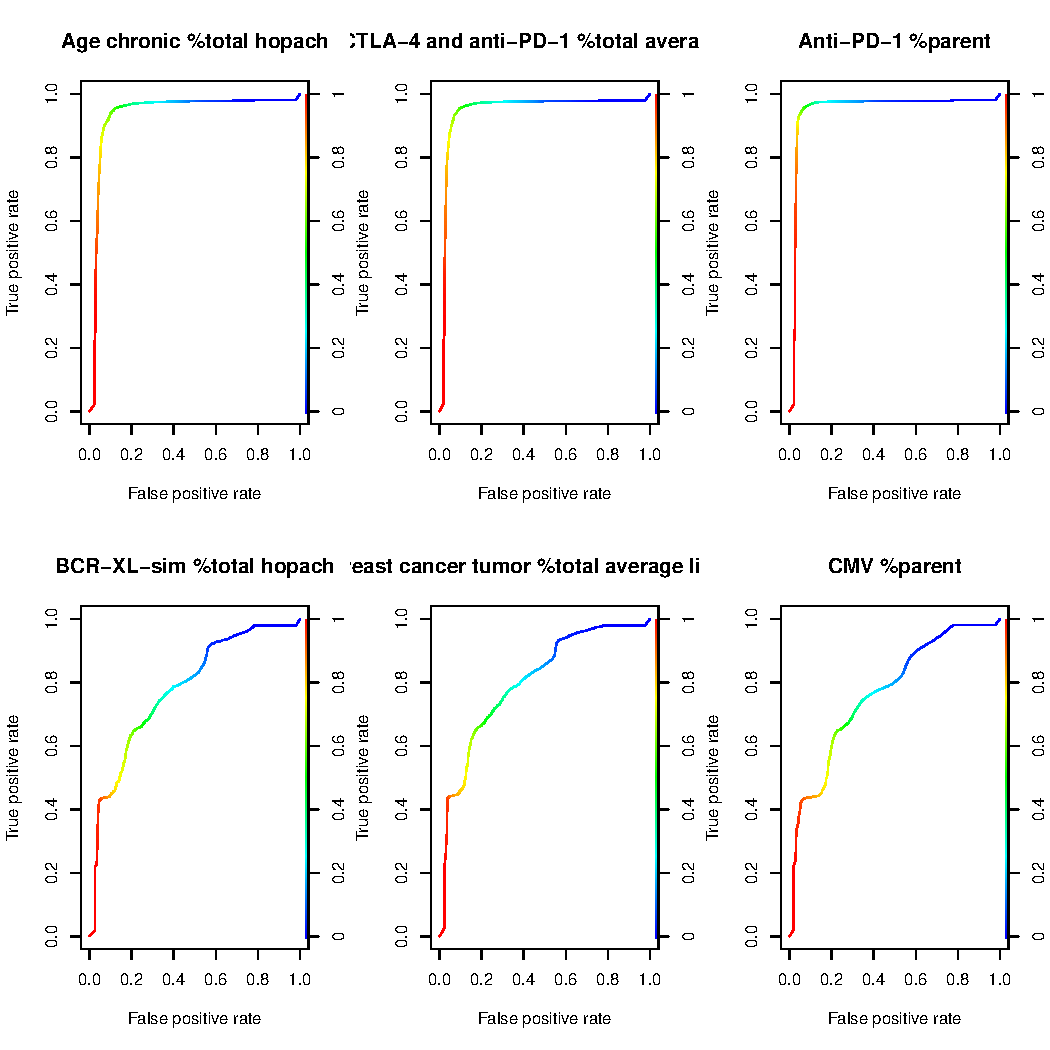
\includegraphics[width=\maxwidth]{figure/ch04_figunnamed-chunk-1-1} 

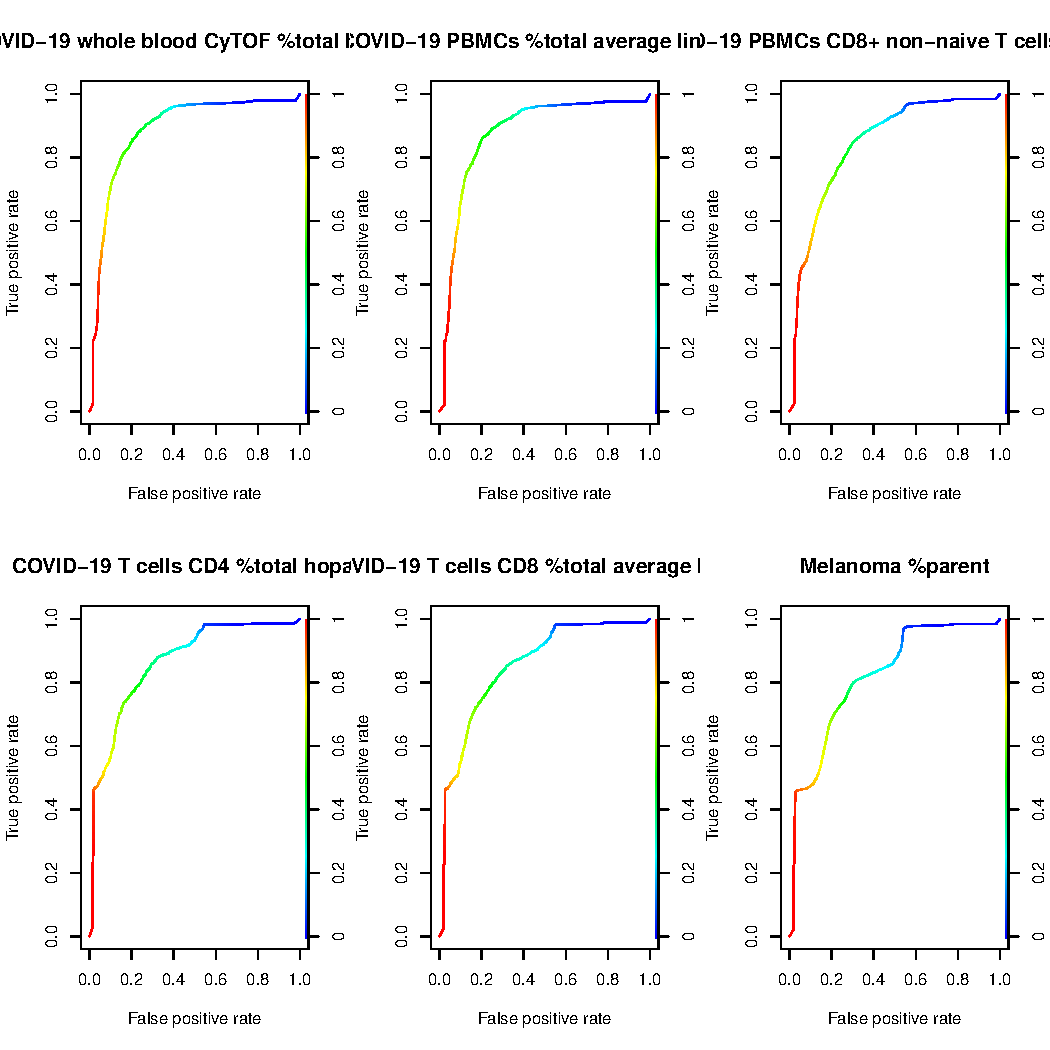
\includegraphics[width=\maxwidth]{figure/ch04_figunnamed-chunk-1-2} 

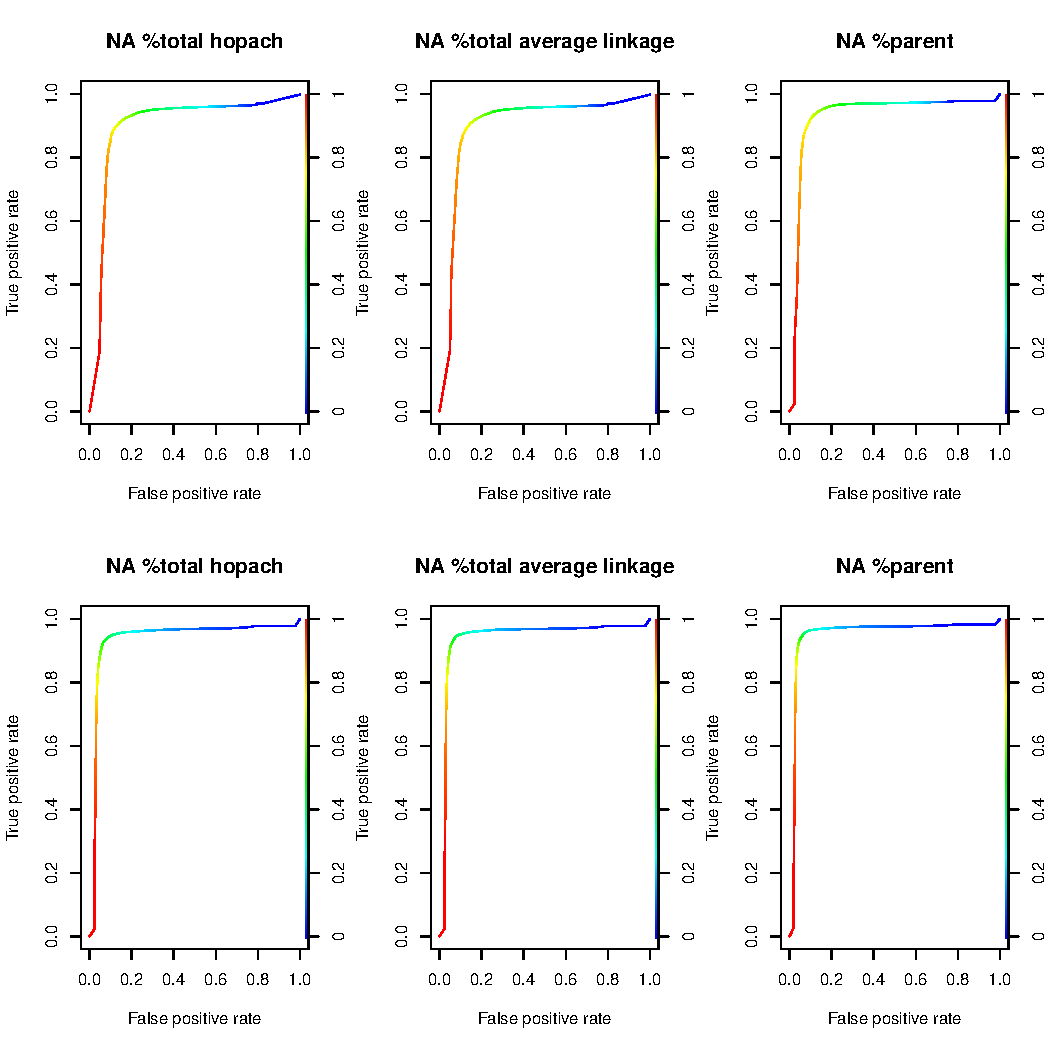
\includegraphics[width=\maxwidth]{figure/ch04_figunnamed-chunk-1-3} 

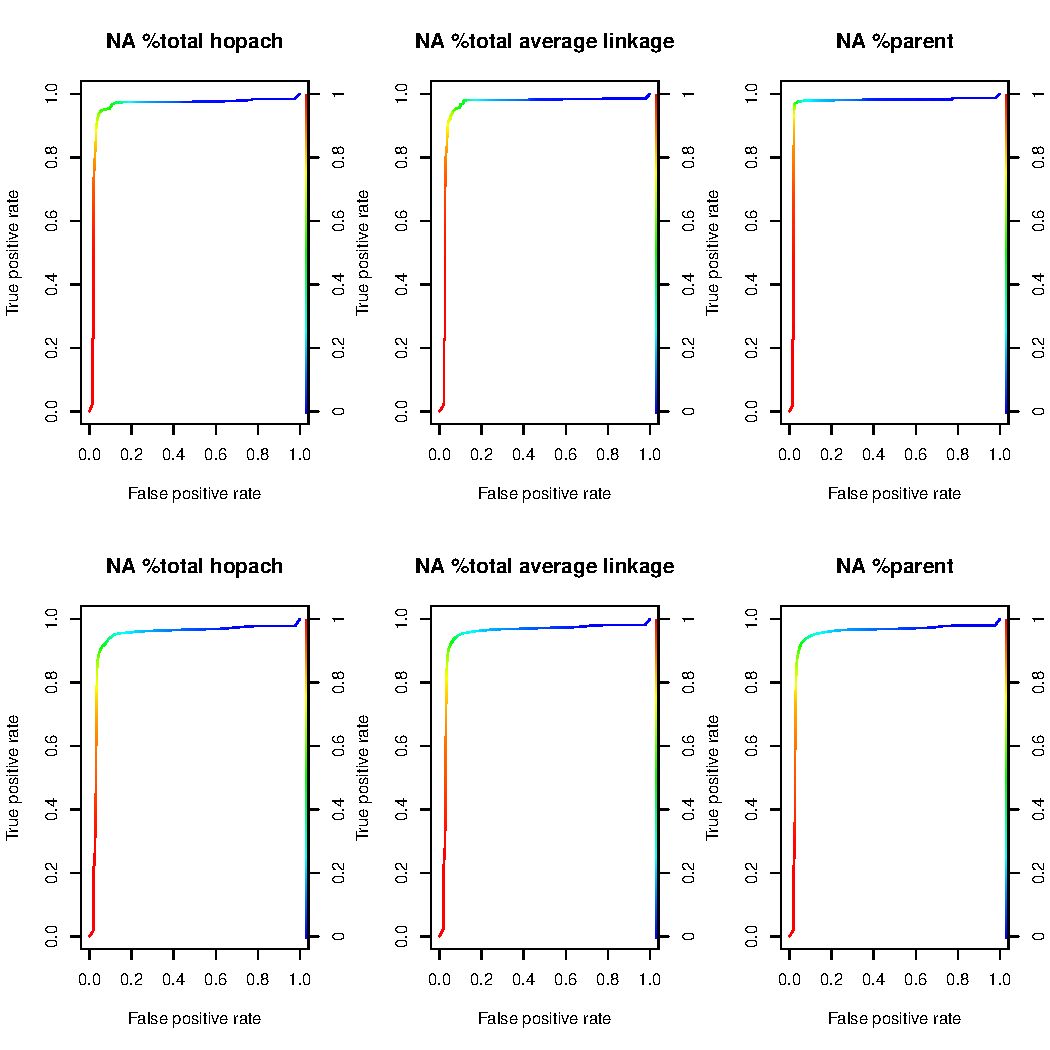
\includegraphics[width=\maxwidth]{figure/ch04_figunnamed-chunk-1-4} 

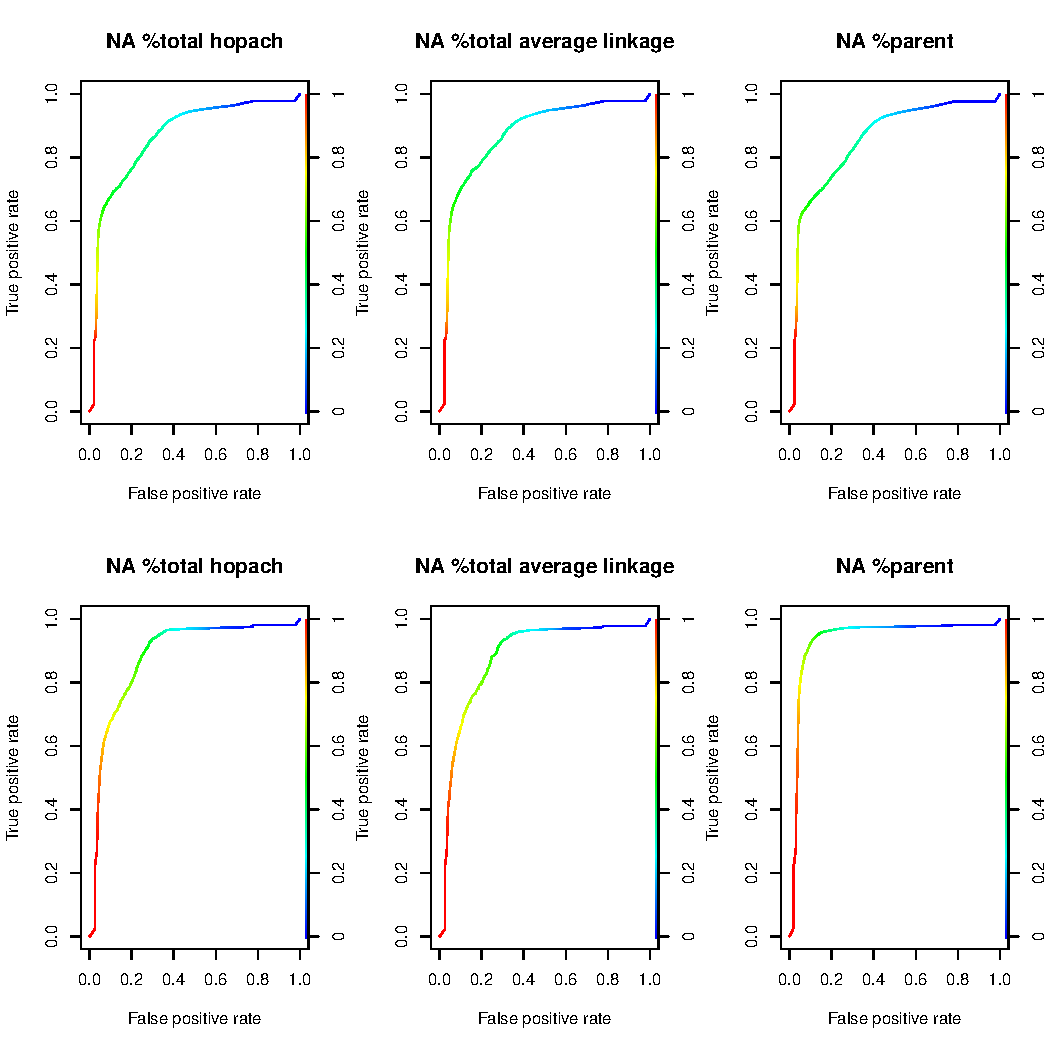
\includegraphics[width=\maxwidth]{figure/ch04_figunnamed-chunk-1-5} 

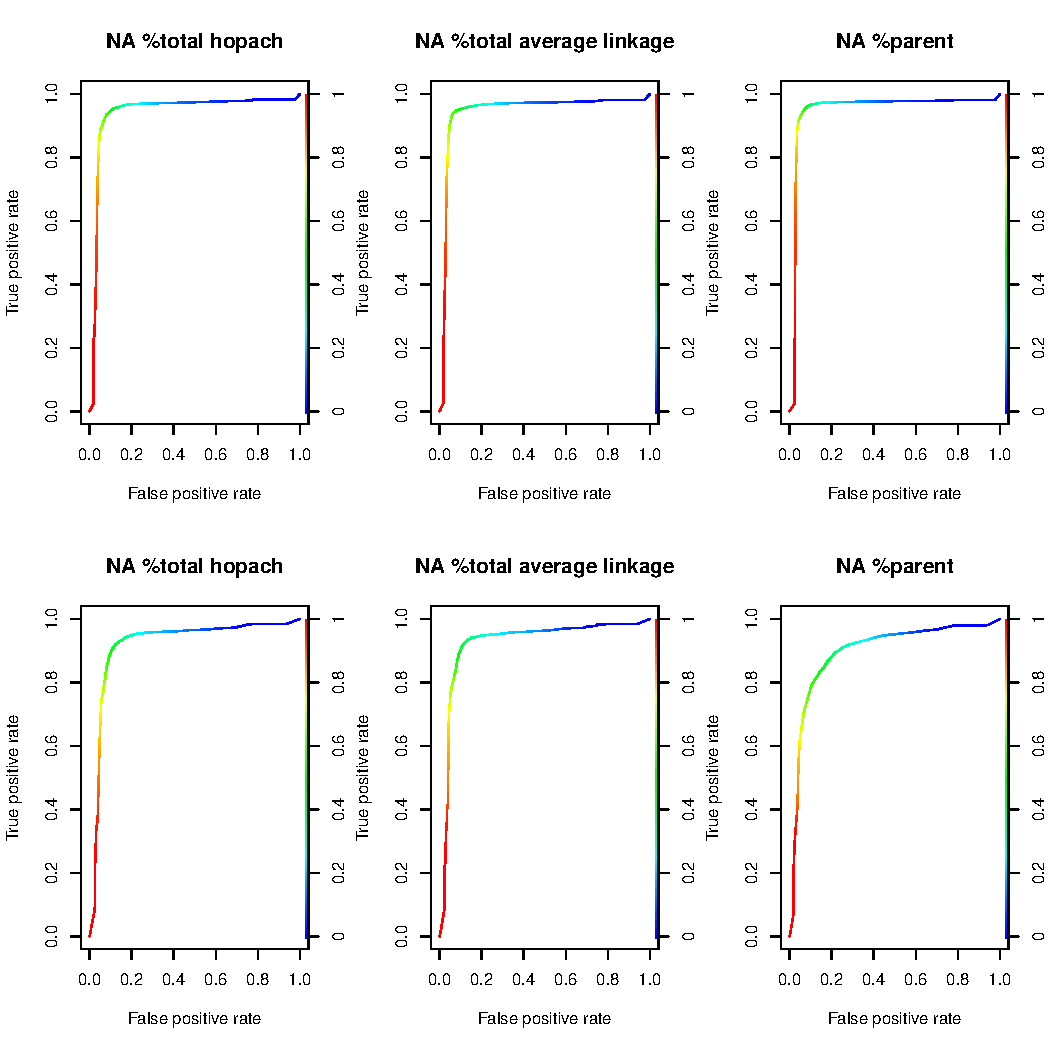
\includegraphics[width=\maxwidth]{figure/ch04_figunnamed-chunk-1-6} 
\end{knitrout}
title{ROC curves.\label{fig:1}}
\end{figure}


- provide Benchmarking plots, once using balanced accuracy as a measure of comparison, once using our "own"
- report findings / observations
